\documentclass[11pt, a4paper]{article}

% ── Codificación y Lenguaje ──────────────────────────────────────────────────
\usepackage[utf8]{inputenc}
\usepackage[T1]{fontenc}
\usepackage[spanish, es-tabla, es-noquoting]{babel}

% ── Geometría ───────────────────────────────────────────────────────────────
\usepackage[top=2.5cm, bottom=2.5cm, left=2.5cm, right=2.5cm, headheight=24pt]{geometry}

% ── Matemáticas ─────────────────────────────────────────────────────────────
\usepackage{amsmath, amssymb, amsthm}
\usepackage{mathtools}

% ── Colores y Cajas ─────────────────────────────────────────────────────────
\usepackage{xcolor}
\usepackage[most]{tcolorbox}
\tcbuselibrary{skins, breakable, theorems}

% ── Tablas ──────────────────────────────────────────────────────────────────
\usepackage{booktabs}
\usepackage{array}
\usepackage{multirow}
\usepackage{longtable}

% ── Listas ──────────────────────────────────────────────────────────────────
\usepackage{enumitem}

% ── Encabezado y Pie de Página ──────────────────────────────────────────────
\usepackage{fancyhdr}

% ── Secciones ───────────────────────────────────────────────────────────────
\usepackage{titlesec}

% ── Gráficos y Diagramas ────────────────────────────────────────────────────
\usepackage{tikz}
\usetikzlibrary{shapes.geometric, arrows.meta, positioning, calc}
\usepackage{graphicx}

% ── Columnas múltiples (formulario) ─────────────────────────────────────────
\usepackage{multicol}

% ── Espaciado ───────────────────────────────────────────────────────────────
\usepackage{setspace}
\setlength{\parskip}{4pt}
\setlength{\parindent}{0pt}

% ── Paleta GOP ──────────────────────────────────────────────────────────────
\definecolor{gopblue}{RGB}{31, 78, 121}
\definecolor{gopcyan}{RGB}{70, 130, 180}
\definecolor{gopgreen}{RGB}{0, 100, 0}
\definecolor{gopgreenlight}{RGB}{230, 255, 230}
\definecolor{goporange}{RGB}{200, 100, 0}
\definecolor{goporangelight}{RGB}{255, 245, 210}
\definecolor{gopred}{RGB}{160, 0, 0}
\definecolor{gopredlight}{RGB}{255, 230, 230}
\definecolor{gopgray}{RGB}{90, 90, 90}
\definecolor{gopgraylight}{RGB}{245, 245, 240}
\definecolor{gopbluedef}{RGB}{0, 70, 140}
\definecolor{gopbluedeflight}{RGB}{220, 235, 255}

% ── Hipervínculos y TOC ─────────────────────────────────────────────────────
\usepackage[colorlinks=true, linkcolor=gopblue, urlcolor=gopblue]{hyperref}

% ── Entornos tcolorbox ───────────────────────────────────────────────────────
\newtcolorbox{definicion}[1]{
  enhanced, breakable,
  colback=gopbluedeflight, colframe=gopbluedef,
  fonttitle=\bfseries\small, title={Definicion: #1}, coltitle=white,
  attach boxed title to top left={yshift=-2mm, xshift=6pt},
  boxed title style={colback=gopbluedef, colframe=gopbluedef, sharp corners},
  sharp corners=south, top=4mm, before skip=6pt, after skip=6pt,
}
\newtcolorbox{formulas}[1]{
  enhanced, breakable,
  colback=gopgreenlight, colframe=gopgreen,
  fonttitle=\bfseries\small, title={Formulas: #1}, coltitle=white,
  attach boxed title to top left={yshift=-2mm, xshift=6pt},
  boxed title style={colback=gopgreen, colframe=gopgreen, sharp corners},
  sharp corners=south, top=4mm, before skip=6pt, after skip=6pt,
}
\newtcolorbox{tipprueba}[1]{
  enhanced, breakable,
  colback=goporangelight, colframe=goporange,
  fonttitle=\bfseries\small, title={TIP PRUEBA: #1}, coltitle=white,
  attach boxed title to top left={yshift=-2mm, xshift=6pt},
  boxed title style={colback=goporange, colframe=goporange, sharp corners},
  sharp corners=south, top=4mm, before skip=6pt, after skip=6pt,
}
\newtcolorbox{trampa}[1]{
  enhanced, breakable,
  colback=gopredlight, colframe=gopred,
  fonttitle=\bfseries\small, title={TRAMPA/ADVERTENCIA: #1}, coltitle=white,
  attach boxed title to top left={yshift=-2mm, xshift=6pt},
  boxed title style={colback=gopred, colframe=gopred, sharp corners},
  sharp corners=south, top=4mm, before skip=6pt, after skip=6pt,
}
\newtcolorbox{ejercicio}[1]{
  enhanced, breakable,
  colback=gopgraylight, colframe=gopgray,
  fonttitle=\bfseries\small\color{black}, title={Ejercicio: #1},
  attach boxed title to top left={yshift=-2mm, xshift=6pt},
  boxed title style={colback=gopgray!40, colframe=gopgray, sharp corners},
  sharp corners=south, top=4mm, before skip=6pt, after skip=6pt,
}
\newtcolorbox{resumentemario}{
  enhanced,
  colback=gopbluedeflight, colframe=gopbluedef,
  fonttitle=\bfseries, title={Resumen del Temario}, coltitle=white,
  attach boxed title to top left={yshift=-2mm, xshift=6pt},
  boxed title style={colback=gopbluedef, colframe=gopbluedef, sharp corners},
}
\newtcolorbox{estructuraprueba}{
  enhanced,
  colback=goporangelight, colframe=goporange,
  fonttitle=\bfseries, title={Estructura de la Prueba}, coltitle=white,
  attach boxed title to top left={yshift=-2mm, xshift=6pt},
  boxed title style={colback=goporange, colframe=goporange, sharp corners},
}
\newtcolorbox{memorizar}{
  enhanced, breakable,
  colback=gopredlight, colframe=gopred,
  fonttitle=\bfseries, title={Conceptos Clave --- Memorizar esto}, coltitle=white,
  attach boxed title to top left={yshift=-2mm, xshift=6pt},
  boxed title style={colback=gopred, colframe=gopred, sharp corners},
  sharp corners=south,
}
\newtcolorbox{paradesarrollo}{
  enhanced, breakable,
  colback=gopgreenlight, colframe=gopgreen,
  fonttitle=\bfseries, title={Para la Etapa Desarrollo (Apuntes Libres Permitidos)}, coltitle=white,
  attach boxed title to top left={yshift=-2mm, xshift=6pt},
  boxed title style={colback=gopgreen, colframe=gopgreen, sharp corners},
  sharp corners=south,
}

% ── Encabezado y pie ─────────────────────────────────────────────────────────
\pagestyle{fancy}
\fancyhf{}
\fancyhead[L]{\small\textbf{GOP ICS3213} --- Examen Final \texttt{2026}}
\fancyhead[C]{}
\fancyhead[R]{\small\nouppercase{\rightmark}}
\fancyfoot[L]{\footnotesize Pronóstico y Preparación Examen}
\fancyfoot[R]{\small\thepage}
\renewcommand{\headrulewidth}{0.4pt}
\renewcommand{\footrulewidth}{0.4pt}

% ── Estilo de secciones ──────────────────────────────────────────────────────
\titleformat{\section}
  {\color{gopblue}\Large\bfseries}{\color{gopblue}\thesection.}{0.5em}{}
  [\color{gopblue}\titlerule]
\titleformat{\subsection}
  {\color{gopblue}\normalsize\bfseries}{\color{gopblue}\thesubsection.}{0.5em}{}
\titleformat{\subsubsection}
  {\color{gopblue}\small\bfseries}{\color{gopblue}\thesubsubsection.}{0.5em}{}

\begin{document}

% ════════════════════════════════════════════════════════════════════════════
% PORTADA
% ════════════════════════════════════════════════════════════════════════════
\begin{titlepage}
  \centering
  \vspace*{2cm}
  {\Huge\bfseries\color{gopcyan} Pronóstico Examen Final\par}
  \vspace{0.4cm}
  {\LARGE\bfseries Gestión de Operaciones\par}
  \vspace{0.3cm}
  {\large ICS3213 --- PUC Chile --- \texttt{2026}\par}
  \vspace{1.2cm}
  \rule{\textwidth}{0.4pt}
  \vspace{0.4cm}

  {\normalsize \texttt{Lunes 6 de Julio de 2026, 8:20 hrs (presencial)}\par}
  \vspace{0.2cm}
  {\small Prof.\ Alejandro Mac Cawley --- Rodrigo Carrasco\par}
  \vspace{0.2cm}
  {\small Salas: Alcalde a Lacámara: K200 | Larrain a Zamorano: K201\par}
  \vspace{0.4cm}
  \rule{\textwidth}{0.4pt}
  \vspace{1cm}

  \begin{resumentemario}
    \begin{itemize}[leftmargin=1.2em, itemsep=2pt]
      \item \textbf{40\% Materia I1 e I2:} MRP, PERT/CPM, Colas y Variabilidad.
      \item \textbf{60\% Materia Nueva:}
      \begin{itemize}[leftmargin=1.2em, itemsep=1pt]
          \item Bodegas y Centros de Distribución
          \item Calidad (Cartas de Control, Capacidad de Proceso)
          \item Coordinación en la cadena (Efecto Látigo, Beer Game)
          \item TPS, Just in Time y Lean Production
          \item Casos: Toyota y Zara
      \end{itemize}
      \item \textbf{La Meta:} Capítulos 27 (inclusive) al final.
    \end{itemize}
  \end{resumentemario}

  \vspace{0.35cm}
  {\small\bfseries\color{gopblue}El potencial de estudiar con IA}\par
  {\footnotesize La IA puede acelerar la exploración, entregar retroalimentación inmediata y
  adaptar la práctica; el aprendizaje se consolida al resolver, contrastar y justificar.}\par
  \vspace{0.1cm}
  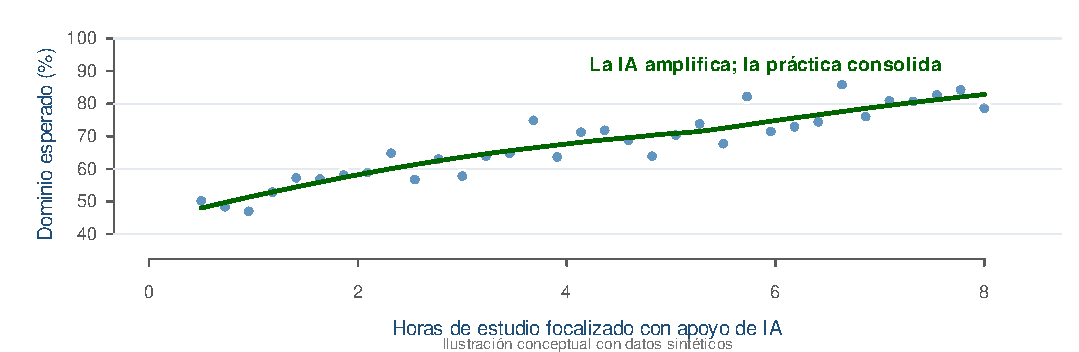
\includegraphics[width=0.50\textwidth]{figuras/potencial_ia.pdf}

  \vspace{0.5cm}

  \begin{estructuraprueba}
    \begin{itemize}[leftmargin=1.2em, itemsep=3pt]
      \item \textbf{Etapa Digital (60 min, SIN apuntes, en CANVAS):}
        \begin{itemize}[leftmargin=1.2em, itemsep=1pt]
          \item 10 preguntas selección múltiple (materia)
          \item 10 preguntas V/F de La Meta (si es Falso, argumentar por qué)
          \item 1 pregunta de desarrollo (Probablemente Casos Toyota/Zara)
        \end{itemize}
      \item \textbf{Descanso de 5 minutos}
      \item \textbf{Etapa Desarrollo (60 min, APUNTES FÍSICOS permitidos):}
        \begin{itemize}[leftmargin=1.2em, itemsep=1pt]
          \item Ejercicios matemáticos y de análisis.
          \item Típicamente 1 problema de Control de Calidad o Localización de Bodegas.
          \item 1 problema de materia anterior (Colas, MRP o PERT).
          \item Escanear y subir a Canvas al final.
        \end{itemize}
    \end{itemize}
  \end{estructuraprueba}

  \vfill
\end{titlepage}

\tableofcontents
\newpage

% ════════════════════════════════════════════════════════════════════════════
\section{Análisis Estratégico y Diagnóstico Probabilístico del Examen}

El examen final de Gestión de Operaciones tiene un formato que premia la \textbf{velocidad conceptual} en la primera hora y la \textbf{precisión de cálculo} en la segunda hora. Para 2026, usamos un modelo de \textbf{prioridad de estudio} que pondera más fuertemente los exámenes recientes (2020: 10\%, 2021: 15\%, 2022: 20\%, 2023: 25\%, 2024: 30\%). Estas cifras son heurísticas: orientan el estudio, pero no garantizan la aparición de una pregunta.

\subsection{Sistema de Diagnóstico Probabilístico (Granular)}

La siguiente tabla fragmenta los temas macro en micro-temas específicos evaluados históricamente, mostrando su aparición real y la probabilidad ponderada proyectada para el examen de 2026.

\vspace{0.3cm}
\begin{table}[h]
\centering
\resizebox{\textwidth}{!}{
\begin{tabular}{l c c c c c c r}
\toprule
\textbf{Micro-Tema Específico} & \textbf{2020} & \textbf{2021} & \textbf{2022} & \textbf{2023} & \textbf{2024} & \textbf{Ocurrencia} & \textbf{Prob. 2026} \\
\midrule
\multicolumn{8}{l}{\textit{\textbf{Bloque 1: Materia de alta prioridad según temario e historial}}} \\
Calidad: Gráficos $\bar{X}$-R y Capacidad & \checkmark & \checkmark & \checkmark & \checkmark & \checkmark & 5/5 & \textbf{100.0 \%} \\
Localización: CG y Break-Even & \checkmark & \checkmark & \checkmark & \checkmark & \checkmark & 5/5 & \textbf{100.0 \%} \\
Colas: Variabilidad, Kingman, VUT & \checkmark & \checkmark & \checkmark & \checkmark & \checkmark & 5/5 & \textbf{100.0 \%} \\
\midrule
\multicolumn{8}{l}{\textit{\textbf{Bloque 2: Materia Rotativa de Desarrollo}}} \\
Inv: MRP, Loteo, Silver-Meal & -- & -- & \checkmark & \checkmark & \checkmark & 3/5 & \textbf{75.0 \%} \\
Opt: Modelamiento MILP & -- & \checkmark & \checkmark & \checkmark & -- & 3/5 & \textbf{60.0 \%} \\
Proy: PERT/CPM y Crashing & -- & \checkmark & -- & \checkmark & -- & 2/5 & \textbf{40.0 \%} \\
\midrule
\multicolumn{8}{l}{\textit{\textbf{Bloque 3: Etapa Digital (Teoría y Casos)*}}} \\
TPS, Kanban, Mudas, Jidoka & \checkmark & \checkmark & \checkmark & \checkmark & \checkmark & 5/5 & \textbf{100.0 \%} \\
Casos: Zara, Toyota, La Meta & \checkmark & \checkmark & \checkmark & \checkmark & \checkmark & 5/5 & \textbf{100.0 \%} \\
\bottomrule
\end{tabular}
}

\vspace{0.15cm}
\footnotesize{* Modelo de peso exponencial: $W_{2020}=0.1, W_{2021}=0.15, W_{2022}=0.2, W_{2023}=0.25, W_{2024}=0.3$. La Etapa Digital sí está explícita en el temario; la tabla no predice la pregunta exacta ni su ponderación interna.}
\end{table}
\vspace{0.3cm}

\begin{tipprueba}{Táctica para la Etapa Digital (CANVAS)}
\begin{enumerate}
    \item \textbf{La Meta (V/F) - 100\% Seguro:} Las preguntas FALSAS requieren argumentación. Sé directo y usa vocabulario del libro (ej. \textit{``Falso, porque reducir lotes disminuye el Lead Time y reduce el WIP''}). Capítulos 27 al final.
    \item \textbf{Casos y TPS - 100\% Seguro:} Lee rápido pero atento a los distractores. Por ejemplo, confundir \textit{Jidoka} con \textit{Heijunka}. Si preguntan por Zara (90\% prob), menciona: (1) Postponement, (2) Integración Vertical, (3) Escasez artificial.
\end{enumerate}
\end{tipprueba}

\begin{tipprueba}{Táctica para la Etapa de Desarrollo}
\begin{enumerate}
    \item \textbf{Calidad (prioridad alta):} Anota datos de promedios y recorridos. \textbf{OJO:} Al sacar muestras atípicas, \textbf{debes recalcular la media y desviación estándar} con las muestras restantes para ver si ahora el proceso está bajo control.
    \item \textbf{Localización (prioridad alta):} Te pueden dar coordenadas o costos. Si piden el punto de indiferencia entre plantas, iguala los Costos Totales. Si la demanda crece en el tiempo ($Q(t)$), integra los costos a lo largo de $T$ años, cuidando si el costo fijo es único o periódico.
    \item \textbf{El Bloque Rotativo (40\% Variante):} Como indica la tabla, hay una lucha muy cerrada entre PERT (55\%), MRP/Loteo (55\%) y Variabilidad (45\%). No puedes descuidar ninguno, pero históricamente cuando sale Variabilidad, suele venir acompañado de un Modelamiento MILP simple.
\end{enumerate}
\end{tipprueba}


\newpage
\section{Sección 1: Control de Calidad Estadístico}

\subsection{Fundamentos Teóricos: Constantes de Control ($A_2, D_3, D_4$)}
En el control estadístico de procesos, estimar la desviación estándar ($\sigma$) directamente a partir de múltiples muestras grandes resulta ineficiente. Por consiguiente, la literatura estadística establece el uso de la \textbf{Tabla de Constantes para Gráficos de Control}.
Estas constantes ($A_2, D_3, D_4$) son factores de conversión matemáticos derivados de la distribución normal. Al multiplicar el Rango Promedio ($\bar{R}$) por estos factores, se obtienen empíricamente los límites de control equivalentes a $3\sigma$.
\begin{itemize}
    \item \textbf{$A_2$}: Factor utilizado para determinar los límites de control del \textbf{Promedio} (Gráfico $\bar{X}$).
    \item \textbf{$D_3$ y $D_4$}: Factores utilizados para determinar el límite inferior y superior, respectivamente, del \textbf{Rango} (Gráfico R).
\end{itemize}

A modo de referencia, la siguiente tabla resume los valores estándar utilizados en los problemas de evaluación:
\begin{center}
\begin{tabular}{cccc}
\toprule
\textbf{Tamaño de Muestra ($n$)} & \textbf{$A_2$} & \textbf{$D_3$} & \textbf{$D_4$} \\
\midrule
5 & 0.577 & 0 & 2.114 \\
10 & 0.308 & 0.223 & 1.777 \\
20 & 0.180 & 0.415 & 1.585 \\
\bottomrule
\end{tabular}
\end{center}

\textbf{Consideración Crítica:} Las constantes deben seleccionarse estrictamente en función de $n$ (tamaño individual de cada muestra extraída), y no en función de $m$ (número total de grupos de muestras analizados).

\begin{tcolorbox}[colback=blue!5!white,colframe=blue!60!black,title=Parámetros del Modelo]
\textbf{Variables Fundamentales:}\\
$m$: Número total de muestras extraídas para el estudio.\\
$n$: Tamaño específico de cada muestra extraída.
\end{tcolorbox}

\subsection{Algoritmo 1: Construcción de Gráficos de Control $\bar{X}$-R}
Procedimiento estructurado para la evaluación:

\begin{enumerate}
    \item \textbf{Calcular Promedios Base:}
    \begin{itemize}
        \item Saca el promedio de promedios: $\bar{\bar{X}} = \frac{\sum \bar{X}_i}{m}$
        \item Saca el promedio de los rangos: $\bar{R} = \frac{\sum R_i}{m}$
    \end{itemize}
    \item \textbf{Leer Tabla de Constantes:} Busca la fila correspondiente a tu \textbf{$n$} (ej. si sacaron 5 tornillos por hora, $n=5$). Extrae $A_2, D_3, D_4$.
    \item \textbf{Calcular Límites de Control:}
    \begin{itemize}
        \item \textbf{Carta $\bar{X}$:} $LCS = \bar{\bar{X}} + A_2 \bar{R}$ \hspace{1cm} $LCI = \bar{\bar{X}} - A_2 \bar{R}$
        \item \textbf{Carta R:} $LCS = D_4 \bar{R}$ \hspace{1.3cm} $LCI = D_3 \bar{R}$
    \end{itemize}
    \item \textbf{Test de Fuera de Control:} Revisa si algún $\bar{X}_i$ o $R_i$ original se sale de sus respectivos límites.
    \item \textbf{EL RECÁLCULO (Casi siempre lo piden):} Si la muestra 3 se salió de los límites y te dicen que fue por una "causa asignable", \textbf{DEBES ELIMINARLA}.
    \begin{itemize}
        \item Nuevo $\bar{\bar{X}} = \frac{(\text{Suma original de } \bar{X}) - \bar{X}_3}{m - 1}$
        \item Nuevo $\bar{R} = \frac{(\text{Suma original de } R) - R_3}{m - 1}$ \\
        \textit{(Aclaración: Como cada $R_i = \text{Máx}_i - \text{Mín}_i$, restar el $R_i$ de la muestra eliminada a la suma de rangos es matemáticamente idéntico a recalcular restando el Máx y Mín de esa muestra de las sumatorias originales).}
        \item Repite el Paso 3 con los nuevos promedios. (Los límites se ajustarán y se harán más estrechos).
    \end{itemize}
\end{enumerate}

\vspace{0.4cm}
\begin{ejercicio}{Gráficos de Control $\bar{X}$-R (Examen 2024 - PII.b)}
\textbf{Enunciado:} Usted controla un proceso de botellas de vidrio. Toma 25 grupos de muestra ($m=25$), cada una de tamaño 20 ($n=20$). Los resultados se detallan a continuación:

\begin{center}
\scriptsize
\begin{tabular}{cccccc|cccccc}
\toprule
\textbf{Muestra} & \textbf{$\bar{X}_i$} & \textbf{Mín} & \textbf{Máx} & \textbf{$R_i$} & & \textbf{Muestra} & \textbf{$\bar{X}_i$} & \textbf{Mín} & \textbf{Máx} & \textbf{$R_i$} \\
\midrule
1 & 25.6 & 24.2 & 27.0 & 2.7 & & 14 & 25.4 & 24.5 & 26.3 & 1.8 \\
2 & 25.7 & 24.1 & 27.2 & 3.1 & & 15 & 25.1 & 24.2 & 26.0 & 1.7 \\
3 & 25.4 & 23.9 & 26.9 & 3.0 & & 16 & 27.5 & 26.2 & 28.8 & 2.6 \\
4 & 25.2 & 23.6 & 26.8 & 3.3 & & 17 & 25.1 & 24.0 & 26.2 & 2.2 \\
5 & 25.5 & 24.8 & 26.2 & 1.5 & & 18 & 25.3 & 24.6 & 26.1 & 1.5 \\
6 & 25.3 & 24.4 & 26.2 & 1.9 & & 19 & 25.4 & 24.2 & 26.5 & 2.3 \\
7 & 25.1 & 23.8 & 26.5 & 2.7 & & 20 & 25.2 & 23.8 & 26.6 & 2.9 \\
8 & 25.2 & 23.9 & 26.5 & 2.6 & & 21 & 25.3 & 24.5 & 26.1 & 1.6 \\
9 & 25.5 & 24.6 & 26.4 & 1.7 & & 22 & 27.6 & 26.3 & 28.9 & 2.6 \\
10 & 25.2 & 24.1 & 26.3 & 2.2 & & 23 & 25.4 & 24.0 & 26.8 & 2.7 \\
11 & 25.1 & 24.0 & 26.2 & 2.3 & & 24 & 25.3 & 24.6 & 26.1 & 1.5 \\
12 & 25.2 & 23.7 & 26.7 & 3.0 & & 25 & 25.1 & 23.7 & 26.6 & 2.9 \\
13 & 25.4 & 24.0 & 26.8 & 2.7 & & & & & & \\
\bottomrule
\end{tabular}
\end{center}

\textit{Nota de desarrollo:} Los valores de Promedio corresponden analíticamente a $\bar{X}_i$ para cada muestra, mientras que el Rango ($R_i$) se obtiene explícitamente calculando $\text{Máx} - \text{Mín}$ en cada fila.

Se entregan las sumas consolidadas: $\sum \bar{X}_i = 637.1$, $\sum \text{Mín} = 607.6$, $\sum \text{Máx} = 666.6$.

Adicionalmente, el enunciado le adjunta la siguiente \textbf{Tabla de Constantes Estadísticas}:
\begin{center}
\scriptsize
\begin{tabular}{cccc}
\toprule
\textbf{Tamaño de Muestra ($n$)} & \textbf{$A_2$} & \textbf{$D_3$} & \textbf{$D_4$} \\
\midrule
5 & 0.577 & 0 & 2.114 \\
10 & 0.308 & 0.223 & 1.777 \\
15 & 0.223 & 0.347 & 1.653 \\
20 & 0.180 & 0.415 & 1.585 \\
25 & 0.153 & 0.459 & 1.541 \\
\bottomrule
\end{tabular}
\end{center}

\textbf{Pregunta (a):} Determine los límites de control del grosor de la botella.

\textbf{Resolución paso a paso según el Algoritmo:}
\begin{enumerate}
    \item \textbf{Promedios Base:} 
    El Promedio General ($\bar{\bar{X}}$) es: $637.1 / 25 = 25.484$.
    Para el Rango Promedio ($\bar{R}$), podemos sumar directamente los $R_i$ de la tabla, o utilizar las sumas consolidadas: $\sum \text{Máx} - \sum \text{Mín} = 666.6 - 607.6 = 59.0$. Luego, $\bar{R} = 59.0 / 25 = 2.36$.
    \item \textbf{Tabla de Constantes:} Dado que el enunciado estipula explícitamente que cada grupo individual posee un tamaño de $n=20$, nos dirigimos a la Tabla de Constantes de la subsección anterior. Ubicando la fila correspondiente a $n=20$, extraemos directamente: $A_2 = 0.18$, $D_3 = 0.415$, $D_4 = 1.585$. (Observación: Es un error conceptual grave utilizar $m=25$ para buscar en dicha tabla).
    \item \textbf{Límites (Gráfico $\bar{X}$):} 
    $LCS = \bar{\bar{X}} + A_2 \cdot \bar{R} = 25.484 + (0.18 \cdot 2.36) = 25.9$.
    $LCI = \bar{\bar{X}} - A_2 \cdot \bar{R} = 25.484 - (0.18 \cdot 2.36) = 25.06$.
    \item \textbf{Límites (Gráfico R):}
    $LCS = D_4 \cdot \bar{R} = 1.585 \cdot 2.36 = 3.74$.
    $LCI = D_3 \cdot \bar{R} = 0.415 \cdot 2.36 = 0.98$.
    \item \textbf{Recálculo y Control Final:}
    Se debe inspeccionar la tabla buscando muestras con un promedio ($\bar{X}_i$) fuera del intervalo matemático aceptable $[25.06, 25.9]$.
    Revisando la columna $\bar{X}_i$: La Muestra 16 ($27.5$) y la Muestra 22 ($27.6$) escapan de los límites definidos.
    \textbf{Acción Correctiva:} Se deben suprimir estas dos observaciones atípicas. Consecuentemente, se restan sus promedios y rangos a las sumatorias originales, se reduce el tamaño del estudio a $m=23$, y se iteran nuevamente los cálculos de los límites:
    \begin{itemize}
        \item Nueva suma $\bar{X}_i$: $637.1 - 27.5 - 27.6 = 582.0$ \hspace{0.5cm} $\rightarrow$ \hspace{0.5cm} Nuevo $\bar{\bar{X}} = 582.0 / 23 = 25.304$
        \item Nueva suma $R_i$: $59.0 - 2.6 - 2.6 = 53.8$ \hspace{0.9cm} $\rightarrow$ \hspace{0.5cm} Nuevo $\bar{R} = 53.8 / 23 = 2.339$
        \item Constantes para $n=20$: Se mantienen inalterables ($A_2 = 0.18$, $D_3 = 0.415$, $D_4 = 1.585$).
        \item \textbf{Nuevos Límites $\bar{X}$:} $LCS = 25.304 + (0.18 \cdot 2.339) = 25.725$ y $LCI = 25.304 - (0.18 \cdot 2.339) = 24.883$
        \item \textbf{Nuevos Límites R:} $LCS = 1.585 \cdot 2.339 = 3.707$ y $LCI = 0.415 \cdot 2.339 = 0.971$
    \end{itemize}
    \textit{Conclusión:} Al inspeccionar nuevamente la tabla, todas las 23 muestras restantes poseen promedios dentro de $[24.883, 25.725]$ y rangos dentro de $[0.971, 3.707]$. El proceso ahora se considera estadísticamente bajo control.
\end{enumerate}
\end{ejercicio}

\subsection{Algoritmo 2: Capacidad de Proceso ($C_p$ y $C_{pk}$)}
Esto mide si tu máquina, aunque esté controlada, es capaz de cumplir lo que pide el cliente (Especificaciones $ES, EI$).

\textbf{Constante de Capacidad ($d_2$):}
Al igual que en los gráficos de control, la estimación de la variabilidad requiere una constante estadística tabulada. El examen proveerá la constante $d_2$ en función del tamaño de muestra $n$.
\begin{center}
\scriptsize
\begin{tabular}{cc}
\toprule
\textbf{Tamaño de Muestra ($n$)} & \textbf{$d_2$} \\
\midrule
5 & 2.326 \\
10 & 3.078 \\
15 & 3.472 \\
20 & 3.735 \\
25 & 3.931 \\
\bottomrule
\end{tabular}
\end{center}

\begin{enumerate}
    \item Calcula la desviación estándar del proceso: $\hat{\sigma} = \frac{\bar{R}}{d_2}$ (buscando $d_2$ en la tabla con tamaño $n$).
    \item Calcula el $C_p$ (Capacidad Potencial sin importar centrado):
    $$ C_p = \frac{ES - EI}{6 \hat{\sigma}} $$
    Si $C_p < 1$, tu máquina es físicamente incapaz de cumplir el ancho pedido, incluso si estuviera perfectamente centrada. \\
    \textit{(Excepción de Examen: Si el problema tiene un solo límite, por ejemplo ``debe resistir al menos 90 grados y no hay máximo'', significa que el garaje está abierto por un lado y su ancho es infinito. Por ende, evaluar si tu auto ``cabe'' adentro ($C_p$) pierde sentido matemático y no se calcula. En este escenario, toda la evaluación de calidad recae de forma absoluta sobre el $C_{pk}$, quien se encargará de medir qué tan lejos estás de chocar con la única pared que sí existe).}
    \item Calcula el $C_{pk}$ (Capacidad Real, castiga el desvío del centro):
    $$ C_{pk} = \min \left( \frac{ES - \bar{\bar{X}}}{3\hat{\sigma}} , \frac{\bar{\bar{X}} - EI}{3\hat{\sigma}} \right) $$
    \textit{(Nota Matemática: ¿Por qué el orden de la resta cambia? Porque las distancias deben ser positivas. Como $ES$ es el techo, restamos $ES - Promedio$. Como $EI$ es el piso, restamos $Promedio - EI$. Si alguna resta te da negativo, significa que el promedio de tu máquina está literalmente operando fuera de las especificaciones del cliente).}
    \item \textbf{Diagnóstico Final (El umbral crítico es 1.0):}
    \begin{itemize}
        \item \textbf{Si $C_{pk} \ge 1$:} La máquina es capaz y está lo suficientemente centrada para no chocar con ninguna pared del garaje.
        \item \textbf{Si $C_{pk} < 1$:} La máquina está produciendo chatarra o defectos (una parte de su curva se sale de los límites).
        \item \textbf{Comparación Clave:} Si tu $C_p \ge 1$ pero tu $C_{pk} < 1$, significa que tu máquina tiene el potencial para cumplir, pero falló por estar \textbf{descentrada}. La solución no es comprar una máquina nueva, es simplemente \textit{calibrar} (mover $\bar{\bar{X}}$ al centro exacto entre $ES$ y $EI$).
    \end{itemize}
\end{enumerate}

\begin{tcolorbox}[colback=yellow!5!white,colframe=yellow!75!black,title={Nota Teórica: La conexión con el $3\sigma$ y $6\sigma$}]
En la industria, la ``huella natural'' de cualquier máquina bajo control abarca $6\hat{\sigma}$ de ancho (desde $-3\hat{\sigma}$ hasta $+3\hat{\sigma}$ respecto al centro, cubriendo el $99.73\%$ de su producción normal). Por eso la fórmula del $C_p$ divide la ventana de tolerancia del cliente ($ES - EI$) exactamente por $6\hat{\sigma}$.
\begin{itemize}
    \item \textbf{Proceso $3\sigma$ ($C_p = 1.0$):} La huella de la máquina ($6\hat{\sigma}$) entra \textit{justo} en el espacio del cliente. Apenas cumples.
    \item \textbf{Proceso $6\sigma$ ($C_p = 2.0$):} Tu máquina es tan precisa que la tolerancia del cliente es el doble de ancha que tu huella. Entran $6\hat{\sigma}$ hacia cada lado ($12\hat{\sigma}$ en total). La tasa de falla es minúscula ($3.4$ defectos por millón).
\end{itemize}
\end{tcolorbox}

\begin{tcolorbox}[colback=purple!5!white,colframe=purple!75!black,title={Perspectiva Gerencial: ¿Es siempre necesario el $6\sigma$?}]
Decidir si exigir tolerancias estrictas (un $ES$ y $EI$ muy cerrados) o si invertir millones en reducir la variabilidad natural ($\hat{\sigma}$) es una decisión puramente estratégica basada en el \textbf{Costo de la Calidad}:
\begin{itemize}
    \item \textbf{Estrategia de Tolerancia Cero (No se afloja):} Si fabricas marcapasos cardíacos o turbinas de avión, una falla significa la muerte de una persona y la quiebra por demandas millonarias. El costo de fallar es infinito. Aquí la estrategia obliga a invertir millones de dólares para lograr un $6\sigma$ ($C_p = 2.0$). La tolerancia es estricta y tu máquina debe ser microscópicamente precisa.
    \item \textbf{Estrategia de Tolerancia Flexible (Se afloja estratégicamente):} Si fabricas cucharas de plástico baratas para cumpleaños, a nadie en el mundo le importa si una cuchara mide 2 milímetros más o menos. El costo de fallar es casi cero. Si intentas aplicar $6\sigma$ comprando maquinaria láser para fabricar cucharas, vas a quebrar por sobrecostos. En este caso, el gerente de operaciones estratégicamente ``afloja'' los límites $ES$ y $EI$ (hace la tolerancia más ancha) y acepta vivir con un $C_p$ más modesto.
\end{itemize}
\textit{Conclusión:} Un ingeniero decide aflojar los parámetros de calidad cuando el costo de arreglar y perfeccionar la máquina supera con creces el costo de que un cliente reciba un producto levemente imperfecto.
\end{tcolorbox}

\vspace{0.4cm}
\begin{ejercicio}{Capacidad con ES y EI completos (Basado en Exámenes)}
\textbf{Enunciado:} Un torno CNC fabrica cilindros metálicos. El plano de ingeniería exige que el diámetro sea de $50 \pm 0.5$ mm para encajar en el motor. Una auditoría de calidad determinó que el proceso actualmente tiene un promedio de $\bar{\bar{X}} = 50.2$ mm y una variabilidad natural $\hat{\sigma} = 0.15$ mm.

\textbf{Pregunta:} Calcule $C_p$ y $C_{pk}$. ¿La máquina es capaz de cumplir? De no serlo, ¿cuál es el problema de raíz?

\textbf{Resolución paso a paso según el Algoritmo:}
\begin{enumerate}
    \item \textbf{Identificación de Especificaciones:} 
    El valor ideal es $50$, con $\pm 0.5$. Por ende: 
    Especificación Superior ($ES$) $= 50.5$ mm.
    Especificación Inferior ($EI$) $= 49.5$ mm.
    \item \textbf{Cálculo del $C_p$ (Potencial):}
    $$ C_p = \frac{ES - EI}{6\hat{\sigma}} = \frac{50.5 - 49.5}{6(0.15)} = \frac{1.0}{0.90} \approx 1.11 $$
    \textit{Análisis parcial:} Como $C_p = 1.11 > 1$, la máquina es físicamente capaz. Su huella total ($0.9$ mm) es más pequeña que la ventana del cliente ($1.0$ mm).
    \item \textbf{Cálculo del $C_{pk}$ (Capacidad Real):} Evaluamos la distancia del promedio hacia ambas paredes.
    \begin{align*}
    C_{pk} &= \min\left\{\frac{50.5-50.2}{3(0.15)},
    \frac{50.2-49.5}{3(0.15)}\right\}\\
    &= \min\left\{\frac{0.30}{0.45},\frac{0.70}{0.45}\right\}
    = \min\{0.66,1.55\}=0.66.
    \end{align*}
    \item \textbf{Diagnóstico Final:} 
    Puesto que $C_{pk} = 0.66 < 1$, el proceso actualmente \textbf{está generando piezas defectuosas}. Al contrastarlo con el $C_p$ ($1.11$), nos damos cuenta de que el problema \textbf{no es la variabilidad natural de la máquina}, sino que está gravemente \textbf{descentrada} hacia el límite superior (su promedio de $50.2$ está peligrosamente cerca del techo de $50.5$). La solución operativa es calibrar el torno para bajar el promedio a $50.0$ mm exactos, sin necesidad de cambiar la máquina.
\end{enumerate}
\end{ejercicio}

\vspace{0.4cm}
\begin{ejercicio}{Capacidad sin ES (Examen 2016 - Vasos Térmicos)}
\textbf{Enunciado:} Usted es el titular de una empresa de café preparado. Ha determinado que los vasos térmicos deben tolerar un mínimo de $90^\circ\text{C}$ (Límite Inferior de Especificación, $EI$) para ser seguros. Se toman muestras de recepción de los proveedores en lotes, donde cada grupo de muestreo consta de 5 vasos ($n=5$). El Promedio General de temperatura tolerada extraído del estudio es de $95^\circ\text{C}$ ($\bar{\bar{X}}$) y el Rango Promedio es $\bar{R} = 4.652^\circ\text{C}$.

\textbf{Pregunta:} Evalúe la capacidad del proceso del proveedor utilizando el índice de capacidad real ($C_{pk}$). ¿Es el proveedor capaz de cumplir con las exigencias?

\textbf{Resolución paso a paso según el Algoritmo:}
\begin{enumerate}
    \item \textbf{Cálculo de la Desviación Estándar ($\hat{\sigma}$):} 
    Al igual que en el algoritmo de gráficos, necesitamos transformar el rango en desviación estándar. Ingresamos a la tabla de constantes con el tamaño de muestra $n=5$ y extraemos $d_2 = 2.326$.
    $$ \hat{\sigma} = \frac{\bar{R}}{d_2} = \frac{4.652}{2.326} = 2^\circ\text{C} $$
    \item \textbf{Identificación de Especificaciones:} 
    Promedio del proceso: $\bar{\bar{X}} = 95^\circ\text{C}$. Especificación Inferior: $EI = 90^\circ\text{C}$. 
    Especificación Superior ($ES$): \textbf{No existe} un límite superior (en este contexto industrial, mientras más resista el vaso el calor, mejor para el cliente).
    \item \textbf{Cálculo del $C_{pk}$ (Capacidad Real):} Dado que solo existe una especificación inferior, no podemos calcular $C_p$. El índice $C_{pk}$ se calcula evaluando únicamente la distancia del centro hacia el único límite existente:
    $$ C_{pk} = \frac{\bar{\bar{X}} - EI}{3\hat{\sigma}} = \frac{95 - 90}{3(2)} = \frac{5}{6} \approx 0.833 $$
    \item \textbf{Diagnóstico Final:} 
    Puesto que $C_{pk} = 0.833 < 1$, se concluye matemáticamente que el proceso del proveedor \textbf{no es capaz} de asegurar consistentemente que todos los vasos resistirán al menos $90^\circ\text{C}$. Una fracción significativa de los vasos fallará por debajo de este estándar de seguridad (se derretirán), lo cual justifica las quejas de los clientes. Se debe exigir al proveedor centrar su proceso (aumentar $\bar{\bar{X}}$) o reducir drásticamente su variabilidad ($\bar{R}$).
\end{enumerate}
\end{ejercicio}

\section{Sección 2: Localización y Bodegas (Break-Even \& Gravedad)}

\begin{tcolorbox}[enhanced, breakable, colback=blue!5!white,colframe=blue!60!black,title=Parámetros del Modelo]
\textbf{Variables Fundamentales:}\\
$CF$: Costo Fijo (ej. costo de adquisición, arriendo o instalación).\\
$CV$: Costo Variable unitario (ej. costo de operación por unidad procesada).\\
$X$ o $Q$: Nivel de producción o demanda esperada.\\
$CT$: Costo Total ($CT = CF + CV \cdot X$).
\end{tcolorbox}

\subsection{Algoritmo 1: Centro de Gravedad (aproximación de localización)}
Encontrar la coordenada $(X^*, Y^*)$ que pondera la posición de cada origen o
destino por el volumen que mueve. En el curso se usa como una aproximación
rápida de localización; no debe confundirse con la solución exacta de cualquier
función de distancia.

\begin{enumerate}
    \item Haz una tabla con columnas: Localidad, $X_i$, $Y_i$, Volumen $V_i$.
    \item Calcula la coordenada $X^*$ ponderando los volúmenes:
    $$ X^* = \frac{\sum (X_i \cdot V_i)}{\sum V_i} $$
    \item Calcula la coordenada $Y^*$ de la misma forma:
    $$ Y^* = \frac{\sum (Y_i \cdot V_i)}{\sum V_i} $$
    \item \textbf{Cálculo de Costo Total (Evaluación de la ubicación):} Si te piden evaluar esta nueva ubicación, primero calcula la \textbf{Distancia Manhattan} $d_i$ hacia cada localidad $i$:
    $$ d_i = |X_i - X^*| + |Y_i - Y^*| $$
    Luego, suma el costo de transporte para todas las localidades:
    $$ \text{Costo Total} = \sum_{i} (\text{Costo Unitario} \cdot V_i \cdot d_i) $$
\end{enumerate}

\begin{trampa}{Centro de Gravedad versus distancia Manhattan}
La fórmula del Centro de Gravedad minimiza exactamente una suma de distancias
\emph{cuadráticas} ponderadas bajo sus supuestos habituales. Si el enunciado
define explícitamente costo proporcional a distancia Manhattan
$|x-x_i|+|y-y_i|$, la solución exacta es una \textbf{mediana ponderada} por
coordenada, no necesariamente el promedio ponderado. En una prueba, aplica el
método que pida el enunciado: ``Centro de Gravedad'' implica la fórmula de
$X^*,Y^*$; ``minimizar Manhattan'' implica comparar la función o usar la
mediana ponderada. Si solo solicitan evaluar el costo de una coordenada dada,
recién ahí calcula la distancia Manhattan de cada ruta.
\end{trampa}

\vspace{0.4cm}
\begin{ejercicio}{Cálculo Centro de Gravedad}
\textbf{Enunciado:} Una empresa desea ubicar un nuevo centro de distribución para abastecer tres localidades:
\begin{itemize}
    \item L1: Coordenadas $(10, 20)$, Volumen demandado $V_1 = 200$
    \item L2: Coordenadas $(30, 40)$, Volumen demandado $V_2 = 300$
    \item L3: Coordenadas $(50, 10)$, Volumen demandado $V_3 = 500$
\end{itemize}

\textbf{Resolución:}
\begin{enumerate}
    \item Volumen total: $\sum V_i = 200 + 300 + 500 = 1000$.
    \item Coordenada $X^*$:
    $$ X^* = \frac{10(200) + 30(300) + 50(500)}{1000} = \frac{2000 + 9000 + 25000}{1000} = 36 $$
    \item Coordenada $Y^*$:
    $$ Y^* = \frac{20(200) + 40(300) + 10(500)}{1000} = \frac{4000 + 12000 + 5000}{1000} = 21 $$
    \item \textbf{Costo Total de Transporte (Distancia Manhattan):} Asumimos que el costo de transporte es el mismo para todas las rutas, por ejemplo, un Costo Unitario $= \$2$ por unidad transportada por km. Al tener la misma ponderación de costo para todas las localidades, este valor constante ($2$) sale factorizado de la sumatoria. Primero calculamos las distancias:
    \begin{align*}
        d_1 &= |10 - 36| + |20 - 21| = 26 + 1 = 27 \\
        d_2 &= |30 - 36| + |40 - 21| = 6 + 19 = 25 \\
        d_3 &= |50 - 36| + |10 - 21| = 14 + 11 = 25
    \end{align*}
    $$ \text{CT} = \sum_{i} (\text{Costo}_i \cdot V_i \cdot d_i) = \sum_{i} (2 \cdot V_i \cdot d_i) = 2 \cdot [ (200 \cdot 27) + (300 \cdot 25) + (500 \cdot 25) ] $$
    $$ \text{CT} = 2 \cdot (5400 + 7500 + 12500) = 2 \cdot 25400 = 50800 $$
\end{enumerate}
\textbf{Conclusión:} La coordenada óptima es $(36, 21)$ con un costo total evaluado de $\$50.800$.
\end{ejercicio}
\vspace{0.4cm}

\subsection{Algoritmo 2: Punto de Equilibrio Lineal (Break-Even)}
Tienes dos opciones de plantas o procesos. ¿Cuál conviene más según la cantidad $Q$?

\begin{enumerate}
    \item \textbf{Plantea la ecuación de Costo Total (CT) para cada opción:} 
    $$ CT = CF + CV \cdot Q $$
    ($CF$ = Costo Fijo, $CV$ = Costo Variable).
    \item \textbf{Punto de Indiferencia:} Iguala $CT_A = CT_B$.
    $$ CF_A + CV_A \cdot Q = CF_B + CV_B \cdot Q $$
    \item Despeja $Q^*$. Este es el umbral.
    \item \textbf{Decisión:} Si produces $Q < Q^*$, elige la de \textbf{menor Costo Fijo}. Si produces $Q > Q^*$, elige la de \textbf{menor Costo Variable}.
\end{enumerate}

\subsection{Algoritmo 3: Break-Even Dinámico (Demanda Creciente)}
Si te dicen "la demanda crece con el tiempo, $Q(t) = m \cdot t$", y te preguntan en qué año ($T$) conviene pasarse a la Planta B.

\begin{enumerate}
    \item \textbf{Iguala las sumatorias o integrales de costo:}
    En vez de igualar el $CT$ de un año, igualas el costo acumulado desde el año 0 hasta $T$.
    \item \textbf{Planteamiento Continuo (Integral):}
    $$ \int_{0}^{T} (CF_A + CV_A \cdot Q(t)) dt = \int_{0}^{T} (CF_B + CV_B \cdot Q(t)) dt $$
    Reemplaza $Q(t) = m \cdot t$, integra ambas partes y despeja $T$.
    \item \textit{Hack para saltarse la integral (solo si $CF$ y $CV$ son constantes):}
    La demanda acumulada hasta $T$ es el área de un triángulo: $\text{Acumulado} = \frac{1}{2} m \cdot T^2$.
    Iguala: $CF_A \cdot T + CV_A (\frac{1}{2} m T^2) = CF_B \cdot T + CV_B (\frac{1}{2} m T^2)$. Dividiendo todo por $T$ (ya que $T>0$), puedes despejar $T$ fácilmente.
\end{enumerate}

\begin{trampa}{Costo fijo de compra versus costo fijo periódico}
Antes de integrar, identifica la unidad del costo fijo. Si $CF$ es una compra
única en $t=0$, el costo acumulado es
$CF + CV\int_0^T Q(t)\,dt$; no corresponde multiplicar $CF$ por cada año.
Si el enunciado define $CF$ como costo de operación por período, entonces sí se
integra $CF\,dt$. Cuando una pauta entregue una convención distinta, declárala
explícitamente y úsala de forma consistente en ambas alternativas.
\end{trampa}

\vspace{0.4cm}
\begin{ejercicio}{Punto de Equilibrio Lineal (Examen 2024 - PI.b)}
\textbf{Enunciado:} Usted evalúa dos localizaciones (L1 y L2).
\begin{itemize}
    \item L1: Compra = 10.000, Operación = 25 / unidad.
    \item L2: Compra = 40.000, Operación = 10 / unidad.
\end{itemize}

\textbf{Pregunta (a):} ¿Qué nivel de producción lo deja indiferente entre L1 o L2?

\textbf{Resolución según el Algoritmo 2 (Break-Even):}
\begin{enumerate}
    \item Planteamos Ecuación L1: $CT_1 = 10.000 + 25X$
    \item Planteamos Ecuación L2: $CT_2 = 40.000 + 10X$
    \item Igualamos (Punto de indiferencia): 
    $10.000 + 25X = 40.000 + 10X$
    \item Despejamos: $15X = 30.000 \rightarrow X = 2.000$ unidades.
\end{enumerate}
\textit{Nota del examen:} Para $X < 2000$ conviene L1 (menor costo fijo). Para $X > 2000$ conviene L2 (menor costo variable).
\end{ejercicio}

\vspace{0.4cm}
\begin{ejercicio}{Break-Even Dinámico}
\textbf{Enunciado:} Una planta antigua tiene Costo Fijo = 0 y Costo Variable = \$10/u. Una planta nueva tiene Costo Fijo = \$20.000 y Costo Variable = \$5/u. La demanda acumulada es creciente con el tiempo según la función $Q_{acum}(T) = \frac{1}{2} (100) T^2$ (es decir, $m=100$). 
¿En qué año $T$ conviene económicamente hacer el cambio a la planta nueva?

\textbf{Resolución según el Algoritmo 3:}
\begin{enumerate}
    \item Costo Acumulado Planta Antigua: $CT_{Antigua} = 0 + 10 \cdot Q_{acum}(T) = 10 \cdot (50 T^2) = 500 T^2$
    \item Costo Acumulado Planta Nueva: $CT_{Nueva} = 20.000 \cdot T + 5 \cdot Q_{acum}(T) = 20.000 T + 250 T^2$
    \item Igualamos Costos Acumulados:
    $$ 500 T^2 = 20.000 T + 250 T^2 $$
    $$ 250 T^2 = 20.000 T $$
    \item Como $T > 0$, dividimos por $T$:
    $$ 250 T = 20.000 \quad \rightarrow \quad T = \frac{20.000}{250} = 80 \text{ años.} $$
\end{enumerate}
\end{ejercicio}

\section{Sección 3: Variabilidad y Teoría de Colas (Fórmula VUT / Kingman)}

\begin{tcolorbox}[colback=blue!5!white,colframe=blue!60!black,title=Parámetros Fundamentales]
\textbf{Variables del Sistema:}\\
$p$: Tiempo promedio de procesamiento (Process time).\\
$a$: Tiempo promedio entre llegadas (Arrival time).\\
$\sigma$: Desviación estándar del proceso o llegada.\\
$CV$: Coeficiente de variabilidad ($\sigma / \text{media}$).\\
$u$: Utilización del sistema ($u = p / a$).
\end{tcolorbox}

\subsection{Algoritmo 1: Cálculo de Variabilidad y Disponibilidad}
Procedimiento estándar para evaluación de equipos:

\begin{enumerate}
    \item \textbf{Tasas vs Tiempos:}
    \begin{itemize}
        \item $a = \text{Tiempo medio entre llegadas}$.
        \item $p = \text{Tiempo medio de procesamiento/servicio}$.
    \end{itemize}
    \item \textbf{Coeficientes de Variación (CV):} Es la desviación estándar dividida por el promedio. Mide la volatilidad.
    \begin{itemize}
        \item $CV_a = \frac{\sigma_a}{a}$
        \item $CV_p = \frac{\sigma_p}{p}$
        \item \textit{Ojo:} Si te dicen "Distribución Exponencial", mágicamente $CV = 1$. Si te dicen "Tiempo Constante/Fijo", mágicamente $CV = 0$.
    \end{itemize}
    \item \textbf{Servidores ($m$):} ¿Cuántas cajas o máquinas atienden en paralelo?
    \item \textbf{Utilización ($\rho$):} $\rho = \frac{p}{a \cdot m}$. Si $\rho > 1$, el sistema colapsa (inestable).
\end{enumerate}

\subsection{Algoritmo 2: La Ecuación de Kingman (Fórmula VUT)}
Calcula el Tiempo de Espera en la Cola ($T_q$). Copia y aplica:

$$ T_q = \left( \frac{CV_a^2 + CV_p^2}{2} \right) \cdot \left( \frac{\rho^{\sqrt{2(m+1)} - 1}}{m(1-\rho)} \right) \cdot p $$

\textbf{Anatomía de VUT (Cómo analizarlo):}
\begin{itemize}
    \item $\mathbf{V}$ (Variabilidad): El primer paréntesis. Si reduces las desviaciones estándar, $T_q$ baja directamente.
    \item $\mathbf{U}$ (Utilización): El segundo paréntesis. Es el penalizador. A medida que $\rho \rightarrow 1$, el denominador $(1-\rho) \rightarrow 0$, disparando el tiempo al infinito.
    \item $\mathbf{T}$ (Tiempo): El tercer componente ($p$). Es el factor de escala.
\end{itemize}

\subsection{Algoritmo 3: Ley de Little (Propagación al Sistema Completo)}
Una vez que tienes el $T_q$ de Kingman, puedes sacar todo lo demás al instante.

\begin{enumerate}
    \item \textbf{Tiempo Total en el Sistema ($T$):} Lo que esperó + lo que tardó en ser atendido.
    $$ T = T_q + p $$
    \item \textbf{Inventario en la Cola ($I_q$):} Personas esperando. Multiplica el tiempo por la tasa de llegada ($\lambda = 1/a$).
    $$ I_q = \frac{T_q}{a} $$
    \item \textbf{Inventario Total en el Sistema ($I$):} Personas esperando + personas siendo atendidas.
    $$ I = \frac{T}{a} $$
\end{enumerate}

\vspace{0.4cm}
\begin{ejercicio}{Kingman (VUT) y Ley de Little}
\textbf{Enunciado:} Un cajero de banco atiende a un ritmo promedio de $p = 6$ minutos por cliente, con una desviación estándar $\sigma_p = 3$ minutos. Los clientes llegan con un tiempo medio entre llegadas de $a = 7.5$ minutos por cliente, siguiendo una distribución exponencial (es decir, $\sigma_a = 7.5$ min). Sólo hay un cajero ($m=1$).

\textbf{Resolución:}
\begin{enumerate}
    \item \textbf{Cálculo de CV y Utilización:}
    $$ CV_p = \frac{3}{6} = 0.5 \quad ; \quad CV_a = \frac{7.5}{7.5} = 1.0 \text{ (por ser exponencial)} $$
    $$ \rho = \frac{p}{a \cdot m} = \frac{6}{7.5 \cdot 1} = 0.8 \text{ (Utilización del 80\%)} $$
    \item \textbf{Tiempo de Espera en Cola ($T_q$) usando Kingman VUT:}
    $$ T_q = \left( \frac{1^2 + 0.5^2}{2} \right) \cdot \left( \frac{0.8^{\sqrt{4}-1}}{1(1-0.8)} \right) \cdot 6 $$
    $$ T_q = \left( \frac{1.25}{2} \right) \cdot \left( \frac{0.8^1}{0.2} \right) \cdot 6 = 0.625 \cdot 4 \cdot 6 = 15 \text{ minutos.} $$
    El cliente pasa en promedio 15 minutos solo esperando.
    \item \textbf{Ley de Little ($T$ e $I_q$):}
    \begin{itemize}
        \item Tiempo total en el sistema: $T = T_q + p = 15 + 6 = 21$ minutos.
        \item Inventario en la cola (personas esperando): $I_q = \frac{T_q}{a} = \frac{15}{7.5} = 2$ personas.
    \end{itemize}
\end{enumerate}
\end{ejercicio}

\vspace{0.4cm}
\begin{ejercicio}{Cálculo de Variabilidad (Examen 2024)}
\textbf{Enunciado:} Mides una máquina perfiladora. Promedio de proceso = 12 minutos. Desviación estándar = 2 minutos.
Te ofrecen una máquina nueva: Promedio = 10 minutos. Desviación = 100 segundos.

\textbf{Pregunta (a y b):} Calcule el coeficiente de variabilidad ($CV$) de ambas máquinas.

\textbf{Resolución según el Algoritmo 1:}
\begin{enumerate}
    \item \textbf{Máquina Antigua:}
    Promedio ($p$) = 12 min. Desv = 2 min.
    $CV = \sigma / p = 2 / 12 = 0.167$
    \item \textbf{Máquina Nueva:}
    Cuidado con la trampa de unidades. Desv = 100 seg = 1.67 minutos.
    $CV = 1.67 / 10 = 0.167$
    \item \textit{Conclusión:} Ambas tienen exactamente la misma variabilidad intrínseca.
\end{enumerate}
*(Luego el problema te hace calcular la Disponibilidad $A = \frac{MTTF}{MTTF + MTTR}$, que también da 0.75 para ambas).*
\end{ejercicio}

\section{Sección 4: Gestión de Proyectos, MRP y Modelamiento (MILP)}

\begin{tcolorbox}[colback=blue!5!white,colframe=blue!60!black,title=Parámetros del Modelo]
\textbf{Variables y Notación:}\\
PERT: $t_o$ (optimista), $t_m$ (probable), $t_p$ (pesimista).\\
MRP (Silver-Meal): $K$ (Costo de emisión/setup), $h$ (Costo de mantener inventario).\\
MILP: $X_{ij}$ (Variable continua de decisión), $Y_i$ (Variable binaria de activación).
\end{tcolorbox}

\subsection{Algoritmo 1: Ruta Crítica y Acortamiento (PERT/CPM)}
Procedimiento para la evaluación de proyectos:

\begin{enumerate}
    \item \textbf{Red PERT y Holguras:} 
    \begin{itemize}
        \item Calcula $ES$ (inicio temprano), $EF=ES+TE$, $LF$ (término tardío) y $LS=LF-TE$.
        \item $\text{Holgura}=LS-ES=LF-EF$. Si la holgura es cero, la actividad pertenece a la
        \textbf{ruta crítica}.
    \end{itemize}
    \item \textbf{Cálculo de Varianzas:} 
    $$ \text{Varianza de una Actividad} = \sigma^2 = \left( \frac{Pesimista - Optimista}{6} \right)^2 $$
    \item \textbf{Probabilidad de Terminar (Z):}
    \begin{itemize}
        \item Varianza de la Ruta ($\sigma^2_{ruta}$) = \textbf{SUMA} de las varianzas de las actividades críticas. \textbf{OJO:} Se suman varianzas, ¡NUNCA se suman las desviaciones estándar!
        \item Para un plazo contractual $T_c$:
        $Z = \frac{T_c - \mu_{ruta}}{\sqrt{\sigma^2_{ruta}}}$ y
        $P(T\le T_c)=\Phi(Z)$.
    \end{itemize}
    \item \textbf{Crashing (Acortamiento):} 
    $$ \text{Costo Marginal} = \frac{Costo_{Acelerado} - Costo_{Normal}}{Tiempo_{Normal} - Tiempo_{Acelerado}} $$
    Siempre acelera la actividad de la ruta crítica con menor costo marginal,
    pero solo mientras tenga margen de reducción. Si aparecen dos rutas críticas,
    debes reducir ambas simultáneamente (o escoger una actividad común) para
    acortar el proyecto.
\end{enumerate}

\vspace{0.4cm}
\begin{ejercicio}{Crashing PERT/CPM (Examen 2023 - Parte 1, Pregunta 2)}
\textbf{Enunciado:} Te dan actividades A, B, C, D, E, F con tiempos normales y de crashing.
\textbf{Resolución Crashing (Paso a Paso):} 1) Identificas la ruta crítica (ej. A-C-E). 2) Divides la diferencia de costo normal/acelerado por los días ahorrados para cada una. 3) Si A cuesta \$100/día y C cuesta \$50/día, \textbf{aceleras C} primero. ¡Nunca aceleres actividades fuera de la ruta crítica porque gastas dinero y el proyecto no se acorta!
\end{ejercicio}

\begin{formulas}{Lectura rápida de una red PERT}
En una pasada hacia adelante, una actividad con varios predecesores comienza
cuando termina el último: $ES_j=\max_i EF_i$. En la pasada hacia atrás, su
término tardío queda determinado por el sucesor más exigente:
$LF_i=\min_j LS_j$. No sumes desviaciones estándar: bajo independencia,
$\sigma_P^2=\sum_{i\in\text{ruta crítica}}\sigma_i^2$ y
$\sigma_P=\sqrt{\sigma_P^2}$. Si el plazo está bajo la media, $Z<0$ y la
probabilidad de cumplimiento es menor que $50\%$.
\end{formulas}

\subsection{Algoritmo 2: MRP y Loteo (Silver-Meal)}
Tienes demandas semanales y un costo de pedir (setup $K$) y mantener ($h$).
Primero explota el BOM y calcula los requerimientos brutos del componente a
partir de los \emph{lanzamientos} planificados de sus padres; no uses
directamente las recepciones del producto padre.

\begin{enumerate}
    \item \textbf{Regla del Costo Promedio (Silver-Meal):} Se van agregando demandas al lote de hoy, hasta que el Costo Promedio por Período empiece a AUMENTAR.
    \item \textbf{Paso 1 (Lote para 1 semana):} Costo Total = $K$. Costo Promedio = $K / 1$.
    \item \textbf{Paso 2 (Lote para 2 semanas):} Costo Total = $K + (Demanda_{sem2} \cdot h \cdot 1)$. Costo Prom = Total / 2.
    \item \textbf{Paso 3 (Lote para 3 semanas):} Costo Total = Anterior $+ (Demanda_{sem3} \cdot h \cdot 2)$. Costo Prom = Total / 3.
    \item \textbf{Corte:} Si el Costo Prom del Paso 3 $>$ Costo Prom del Paso 2, detente. El pedido será solo para las semanas 1 y 2. Inicia un nuevo pedido en la semana 3.
    \item \textbf{MRP completo:} La recepción planificada se ubica en el período de necesidad y
    el lanzamiento se desplaza hacia atrás según el lead time:
    $PORelease_{t-L}=POR_t$. Antes de aplicar Silver-Meal descuenta inventario
    disponible y recepciones programadas.
\end{enumerate}

\vspace{0.4cm}
\begin{ejercicio}{Algoritmo Silver-Meal (Examen 2022 / 2024)}
\textbf{Enunciado Loteo:} Setup $K = \$50$. Costo inventario $h = \$2$/semana. Demanda: Sem1=10, Sem2=15, Sem3=5.
\textbf{Resolución Silver-Meal:}
- \textbf{Opción 1 (Pedir solo S1):} Costo Total = 50. Costo Prom = 50 / 1 = \textbf{50}.
- \textbf{Opción 2 (Pedir S1 y S2):} Pido 25 hoy. Guardo 15 para la otra semana. Costo Total = $50 + (15 \times 2 \times 1) = 80$. Costo Prom = 80 / 2 = \textbf{40}.
- \textbf{Opción 3 (Pedir S1, S2, S3):} Pido 30. Costo = $50 + 30 + (5 \times 2 \times 2) = 100$. Costo Prom = 100 / 3 = \textbf{33.3}.
Sigo agregando mientras el Costo Promedio siga bajando.
\end{ejercicio}

\begin{formulas}{Wagner--Whitin: óptimo global}
Cuando el enunciado pida el óptimo exacto, Silver--Meal es solo una heurística.
Con $f(t)$ igual al costo mínimo acumulado hasta el período $t$:
\[
f(t)=\min_{1\le j\le t}\left\{f(j-1)+K+
H\sum_{r=j}^{t}(r-j)D_r\right\},\qquad f(0)=0.
\]
La alternativa $j$ representa emitir en $j$ una orden que cubre las demandas
$j,\ldots,t$. La política óptima se recupera siguiendo hacia atrás las
alternativas que alcanzan el mínimo.
\end{formulas}

\subsection{Algoritmo 3: Modelamiento MILP (Diagnóstico y Formulación)}
Si te piden escribir la función objetivo (F.O.) y las restricciones.
\begin{enumerate}
    \item \textbf{Variables de Decisión:} $X_{ij}$ (Cantidad producida/enviada), $Y_i$ (Binaria 1 si abro planta, 0 si no).
    \item \textbf{Función Objetivo (Minimizar Costos):} Suma del (Costo Unitario $\cdot X_{ij}$) + (Costo Fijo $\cdot Y_i$).
    \item \textbf{Restricción de Demanda:} Todo lo que entra al cliente debe ser $\ge$ Demanda.
    \item \textbf{Restricción Lógica (Capacidad) - ¡La más importante!:}
    $$ \sum X_{ij} \le M \cdot Y_i $$
    (Si $Y_i=0$, obliga a que $X=0$. Si $Y_i=1$, permite operar hasta $M$).
\end{enumerate}

\begin{formulas}{Plantilla completa de localización capacitada}
Para plantas $i\in I$ y clientes $j\in J$, define $x_{ij}\ge0$ como el flujo
enviado y $y_i\in\{0,1\}$ como la apertura de la planta. Con demanda
$D_j$, capacidad $U_i$, costo fijo $F_i$ y costo unitario $c_{ij}$:
\[
\begin{aligned}
\min\quad &\sum_{i\in I}F_i y_i+\sum_{i\in I}\sum_{j\in J}c_{ij}x_{ij}\\
\text{s.a.}\quad &\sum_{i\in I}x_{ij}\ge D_j &&\forall j\in J,\\
&\sum_{j\in J}x_{ij}\le U_i y_i &&\forall i\in I,\\
&x_{ij}\ge0,\quad y_i\in\{0,1\}.
\end{aligned}
\]
Si hay inventario por período, agrega el balance
$I_{t}=I_{t-1}+P_t-D_t$; si hay activación consecutiva, usa una binaria
$z_t\ge y_t-y_{t-1}$ y cobra el costo fijo sobre $z_t$, no sobre todos los
períodos operados.
\end{formulas}

\vspace{0.4cm}
\begin{ejercicio}{Modelamiento MILP (Examen 2021 / 2023 - Parte 2)}
\textbf{Enunciado MILP:} Tienes 3 plantas posibles para abastecer 5 ciudades. Abrir una planta cuesta $F_i$. El transporte cuesta $C_{ij}$. Plantea el modelo de minimización.
\textbf{Resolución (Variables Clave):}
Escribe esto en tu cuaderno:
Binaria $Y_i = 1$ si abro la planta $i$ y continua $X_{ij}$ igual a la
cantidad enviada de la planta $i$ a la ciudad $j$. La función objetivo es
\[
\min Z=\sum_iF_iY_i+\sum_i\sum_j C_{ij}X_{ij},
\]
acompañada por demanda, capacidad y dominio de las variables. Sin estas
restricciones, la expresión anterior no es todavía un modelo MILP completo.
\end{ejercicio}


\newpage
\section{Toyota Production System (TPS) y Lean}

\begin{tcolorbox}[colback=red!5!white,colframe=red!75!black,title=Mapa Mental Rápido (Cópialo)]
\textbf{Filosofía Lean:} Eliminar desperdicios (Mudas) de forma implacable.\\
\textbf{Dos Pilares del TPS:} 
1. \textit{JIT (Just in Time):} Producir solo lo necesario, cuando es necesario (Kanban / Pull).
2. \textit{Jidoka:} Autonomatización con toque humano (Calidad en la fuente, parar la línea si hay error).
\end{tcolorbox}

\subsection{Los 7 Mudas (Desperdicios a evitar)}
Anota y memoriza esta lista, suelen cruzar conceptos en los V/F:
\begin{enumerate}
    \item \textbf{Sobreproducción:} El peor de todos (crea los demás). Hacer más de lo pedido.
    \item \textbf{Inventario:} Oculta los problemas bajo el agua (teoría del barco y las rocas).
    \item \textbf{Movimiento:} Personas moviéndose ineficientemente en su estación.
    \item \textbf{Transporte:} Mover materiales largas distancias innecesariamente.
    \item \textbf{Esperas:} Tiempos muertos de máquinas o personas.
    \item \textbf{Sobre-procesamiento:} Hacer cosas que el cliente no valora ni paga.
    \item \textbf{Defectos:} Reprocesos y fallas de calidad.
\end{enumerate}

\subsection{Conceptos y Herramientas (Vocabulario de Examen)}
\begin{itemize}[itemsep=1ex]
    \item \textbf{Genchi Genbutsu:} Ir a la fuente real del problema. No diagnosticar desde la oficina.
    \item \textbf{Kaizen:} Mejora continua con participación de todos, no solo de gerencia.
    \item \textbf{Heijunka:} Nivelación de la producción en volumen y mix (fabricar un poco de todo cada día, no por lotes masivos).
    \item \textbf{Kanban:} Tarjetas visuales que autorizan la producción. Son el nervio del sistema \textbf{PULL}.
    \item \textbf{Sistema Pull vs Push:} \textit{Pull} (jalar) reacciona a la demanda real. \textit{Push} (empujar) produce basado en pronósticos ciegos (como MRP).
    \item \textbf{Poka-Yoke:} Mecanismo a prueba de errores (ej. un conector que solo encaja de un lado). Apoya a Jidoka.
    \item \textbf{Andon:} Pizarra de luces para pedir ayuda o parar la línea.
    \item \textbf{5S:} Clasificar, ordenar, limpiar, estandarizar y sostener. Es disciplina visual y operacional del puesto de trabajo.
\end{itemize}

\begin{tcolorbox}[colback=blue!5!white,colframe=blue!70!black,title=Historia TPS que puede caer en V/F]
\textbf{Sakichi Toyota:} telar automático que se detenía al detectar falla. Es la raíz de \textbf{Jidoka}: calidad en la fuente y detención ante anomalías.\\
\textbf{Taiichi Ohno:} observa supermercados y desarrolla la lógica de reposición según consumo real: base del \textbf{Just-in-Time} y del sistema \textbf{Pull}.\\
\textbf{TPS no es solo técnica:} también es cultura de mejora continua, respeto, trabajo en equipo y resolución en la fuente.
\end{tcolorbox}

\subsection{Trampas Clásicas (V/F)}
\begin{itemize}
    \item \textit{``Lean significa cero inventario siempre.''} $\rightarrow$ \textbf{FALSO.} El inventario se minimiza, pero se mantiene un "buffer" estratégico para fluidez.
    \item \textit{``Jidoka es producir rápido y revisar la calidad al final.''} $\rightarrow$ \textbf{FALSO.} Es revisar en la fuente y parar inmediatamente.
    \item \textit{``En TPS se prefiere un lote grande para ahorrar setup.''} $\rightarrow$ \textbf{FALSO.} Se reduce el tiempo de setup (SMED) para poder usar lotes mínimos.
    \item \textit{``Heijunka significa producir siempre el mismo producto.''} $\rightarrow$ \textbf{FALSO.} Es nivelar volumen y mezcla para evitar variabilidad y sobrecargas.
    \item \textit{``Andon es solo un tablero informativo.''} $\rightarrow$ \textbf{FALSO.} Es un mecanismo para visibilizar anomalías y activar ayuda/detención.
\end{itemize}

\section{Casos de Estudio (Etapa Digital)}

\begin{tcolorbox}[colback=purple!5!white,colframe=purple!75!black,title=Mapa Mental Rápido (Cópialo)]
\textbf{Zara:} Agilidad extrema, escasez artificial, diseño y producción in-house.\\
\textbf{Barilla:} Efecto Látigo (Bullwhip), variabilidad exagerada de pedidos.\\
\textbf{Hospitales (Virginia Mason):} TPS aplicado a servicios (flujo continuo del paciente).
\end{tcolorbox}

\subsection{Caso Zara (Agilidad en Fast Fashion)}
Este caso evalúa cómo Zara evita los grandes descuentos de la industria de la moda. Anota estos 4 pilares:
\begin{enumerate}
    \item \textbf{Diseño Centralizado:} Decenas de miles de diseños nuevos al año con fuerte feedback diario desde las tiendas (Store Managers).
    \item \textbf{Producción In-House vs Outsourcing:} Las prendas "trendy" (de moda rápida) se fabrican cerca (España/Portugal/Marruecos) para rapidez. Los básicos (ej. poleras blancas) se tercerizan a Asia para costo.
    \item \textbf{Postponement (Pospocisión):} Retrasar el teñido o ensamblaje final hasta conocer qué colores se están vendiendo en tiempo real.
    \item \textbf{Escasez Artificial:} No reponer lo que se agotó. Esto obliga al cliente a comprar inmediatamente ("si no lo llevo ahora, mañana no estará").
\end{enumerate}

\subsection{Caso Barilla (JITD / VMI)}
\begin{itemize}[itemsep=1ex]
    \item \textbf{El Problema:} El \textit{Efecto Látigo} (Bullwhip Effect). Pequeñas variaciones de demanda en tiendas causaban fluctuaciones gigantescas en la fábrica debido a la política de lotes y promociones.
    \item \textbf{La Solución JITD (Just In Time Distribution):} Barilla decide tomar el control del inventario de sus distribuidores. En lugar de recibir "pedidos", Barilla mira el inventario del cliente y le repone solo lo necesario (\textit{Vendor Managed Inventory}).
\end{itemize}

\subsection{Caso Hospital Virginia Mason (TPS en Servicios)}
\begin{itemize}[itemsep=1ex]
    \item \textbf{El Problema:} Médicos perdiendo tiempo buscando insumos, pacientes esperando horas (altos \textit{Mudas}).
    \item \textbf{La Solución (Flujo Continuo):} El paciente no se mueve; los especialistas y equipos orbitan alrededor de él. Uso de "kits" estandarizados de instrumentos. Aplicación directa de TPS a personas.
\end{itemize}

\section{La Meta (Goldratt) - Heurísticas V/F}

\begin{tcolorbox}[colback=blue!5!white,colframe=blue!75!black,title=Mapa Mental Rápido (Cópialo)]
\textbf{Objetivo:} Ganar dinero (Aumentar Throughput $\uparrow$, Bajar Inventario $\downarrow$, Bajar Gasto Operativo $\downarrow$).\\
\textbf{Cuello de Botella (CB):} Recurso con Capacidad $\le$ Demanda (Herbie).\\
\textbf{Regla de Oro:} Una hora ganada en un CB es una hora ganada para el sistema. Una hora ganada en un NO-CB es un espejismo.
\end{tcolorbox}

\subsection{Heurísticas Verdadero / Falso (Trampas Clásicas)}
Anota estas reglas. Si lees lo contrario en el examen, es \textbf{FALSO}.

\begin{itemize}[itemsep=1ex]
    \item \textbf{Sobre Tamaños de Lote:}
    \begin{itemize}
        \item Reducir el lote de transferencia $\rightarrow$ Disminuye el WIP (Inventario en Proceso) y el Lead Time (Tiempo de Flujo).
        \item Reducir el lote $\rightarrow$ \textbf{NO} aumenta el Lead Time (es falso si dice lo contrario).
        \item Los lotes de transferencia \textbf{no} tienen que ser iguales a los lotes de proceso.
    \end{itemize}
    
    \item \textbf{Sobre Cuellos de Botella (CB):}
    \begin{itemize}
        \item Optimizar un recurso no-CB es una pérdida de tiempo y solo genera más inventario (WIP) atascado frente al CB.
        \item El CB dicta el ritmo (Tambor / Drum) de toda la planta.
        \item Si se daña una máquina frente al CB, importa menos que si se daña el propio CB.
    \end{itemize}
    
    \item \textbf{Sobre las Fluctuaciones Estadísticas:}
    \begin{itemize}
        \item Las fluctuaciones y eventos dependientes se acumulan en lugar de promediarse (fenómeno de la excursión de boy scouts).
        \item El último paso de la línea siempre sufrirá los peores retrasos heredados de los procesos anteriores.
    \end{itemize}
\end{itemize}

\subsection{Los 5 Pasos de la Teoría de Restricciones (TOC)}
(Anota el orden exacto, es evaluado siempre):
\begin{enumerate}
    \item \textbf{Identificar} la restricción del sistema (Encontrar a Herbie).
    \item \textbf{Explotar} la restricción (Que Herbie no se detenga por tonterías, quitarle la carga inútil).
    \item \textbf{Subordinar} todo lo demás a la decisión anterior (Los rápidos no deben adelantar a Herbie; sistema de cuerdas).
    \item \textbf{Elevar} la restricción (Comprar otra máquina, contratar más gente para el CB).
    \item \textbf{Volver al paso 1} (Si se rompió la restricción, buscar el nuevo CB. No dejar que la inercia gane).
\end{enumerate}

\section{Coordinación y Efecto Látigo (Canvas)}

\begin{tcolorbox}[colback=cyan!5!white,colframe=cyan!75!black,title=Mapa Mental Rápido (Cópialo)]
\textbf{Efecto Látigo (Bullwhip):} Variación amplificada aguas arriba. Un pequeño cambio en el cliente final genera un caos de pedidos en la fábrica.\\
\textbf{La Solución Maestra:} Compartir el POS (Point of Sale) para que todos vean la demanda real, no los pedidos distorsionados del eslabón anterior.
\end{tcolorbox}

\subsection{Ejercicio Clave de Clase: Doble Marginalización}

\begin{definicion}{Qué está midiendo este ejercicio}
Este ejercicio compara una cadena \textbf{descentralizada} contra una cadena \textbf{centralizada}. En la cadena descentralizada, el proveedor y el minorista maximizan sus propias utilidades por separado. En la cadena centralizada, se maximiza la utilidad total de la cadena completa.

La pérdida de eficiencia aparece porque ambos agentes agregan margen: primero el proveedor sube el precio mayorista \(w\), y luego el minorista sube el precio final \(p\). A esto se le llama \textbf{doble marginalización}.
\end{definicion}

\begin{formulas}{Plantilla del modelo fabricante--minorista}
Demanda inversa:
\[
p=a-bq.
\]
Costo unitario del proveedor:
\[
c.
\]

En la cadena descentralizada, el proveedor elige \(w\) y el minorista elige \(q\). Dado \(w\), el minorista maximiza:
\[
\Pi_r(q)=q(p-w)=q(a-bq-w).
\]
Derivando:
\[
\frac{d\Pi_r}{dq}=a-w-2bq=0
\quad\Rightarrow\quad
q(w)=\frac{a-w}{2b}.
\]
El proveedor anticipa esta respuesta y maximiza:
\[
\Pi_s(w)=(w-c)q(w)
=(w-c)\frac{a-w}{2b}.
\]
Derivando:
\[
\frac{d\Pi_s}{dw}=0
\quad\Rightarrow\quad
w^*=\frac{a+c}{2}.
\]
Por lo tanto:
\[
q_D=\frac{a-c}{4b},
\qquad
p_D=\frac{3a+c}{4}.
\]
Las utilidades descentralizadas son:
\[
\Pi_s^D=\frac{(a-c)^2}{8b},
\qquad
\Pi_r^D=\frac{(a-c)^2}{16b},
\qquad
\Pi_{SC}^D=\frac{3(a-c)^2}{16b}.
\]

En la cadena centralizada, se maximiza la utilidad total:
\[
\Pi_{SC}(q)=q(p-c)=q(a-bq-c).
\]
Derivando:
\[
\frac{d\Pi_{SC}}{dq}=a-c-2bq=0
\quad\Rightarrow\quad
q_C=\frac{a-c}{2b}.
\]
Luego:
\[
p_C=\frac{a+c}{2},
\qquad
\Pi_{SC}^C=\frac{(a-c)^2}{4b}.
\]
\end{formulas}

\begin{ejercicio}{Caso de clase: \(Q=100-P\), \(c=1\)}
El enunciado de clase usa:
\[
Q=100-P
\quad\Leftrightarrow\quad
p=100-q,
\qquad
a=100,\quad b=1,\quad c=1.
\]

\textbf{Cadena descentralizada:}
\[
w_D=\frac{100+1}{2}=50.5,
\]
\[
q_D=\frac{100-1}{4}=24.75,
\qquad
p_D=\frac{3(100)+1}{4}=75.25.
\]
Utilidades:
\[
\Pi_s^D=(50.5-1)(24.75)=1225.125,
\]
\[
\Pi_r^D=(75.25-50.5)(24.75)=612.5625,
\]
\[
\Pi_{SC}^D=1837.6875.
\]

\textbf{Cadena centralizada:}
\[
q_C=\frac{100-1}{2}=49.5,
\qquad
p_C=\frac{100+1}{2}=50.5,
\]
\[
\Pi_{SC}^C=(50.5-1)(49.5)=2450.25.
\]

Comparación:
\[
q_C=49.5>24.75=q_D,
\qquad
p_C=50.5<75.25=p_D,
\]
\[
\Pi_{SC}^C=2450.25>1837.69=\Pi_{SC}^D.
\]
La cadena descentralizada vende menos, cobra más caro y genera menor utilidad total.
\end{ejercicio}

\begin{tipprueba}{Cómo contestarlo rápido}
Si aparece este ejercicio, no partas inventando. Usa esta secuencia:
\[
\text{minorista: } q(w)
\quad\rightarrow\quad
\text{proveedor: } w^*
\quad\rightarrow\quad
\text{descentralizado}
\]
\[
\quad\rightarrow\quad
\text{centralizado}
\quad\rightarrow\quad
\text{comparar}.
\]
La frase final debe decir: ``La falta de coordinación produce doble marginalización; por eso la cadena descentralizada vende menos que el óptimo integrado''.
\end{tipprueba}

\begin{formulas}{Contrato de compartir utilidades}
Una forma de coordinar es un contrato de compartir ingresos/utilidades. Si el minorista conserva una fracción \(\alpha\) de los ingresos y paga \(w\) por unidad, su utilidad es:
\[
\Pi_r(q)=\alpha R(q)-wq.
\]
Para que el minorista elija la cantidad centralizada, debe cumplirse:
\[
R'(q)=c.
\]
Pero el minorista elige según:
\[
\alpha R'(q)-w=0
\quad\Rightarrow\quad
R'(q)=\frac{w}{\alpha}.
\]
Entonces el contrato coordina si:
\[
\frac{w}{\alpha}=c
\quad\Rightarrow\quad
w=\alpha c.
\]
Con \(w=\alpha c\), el minorista recibe:
\[
\Pi_r=\alpha \Pi_{SC}^C,
\]
y el proveedor recibe:
\[
\Pi_s=(1-\alpha)\Pi_{SC}^C.
\]
En el ejemplo:
\[
\Pi_{SC}^C=2450.25.
\]
Para que ambos queden mejor que en el caso descentralizado:
\[
\alpha(2450.25)>612.56
\quad\Rightarrow\quad
\alpha>0.25,
\]
\[
(1-\alpha)(2450.25)>1225.13
\quad\Rightarrow\quad
\alpha<0.50.
\]
Por lo tanto, cualquier:
\[
\boxed{0.25<\alpha<0.50}
\]
mejora a ambos agentes respecto de la cadena descentralizada.
\end{formulas}

\begin{ejercicio}{Interpretación de clase: Blockbuster, Netflix y reparto de ingresos}
El caso Blockbuster/Netflix es la aplicación práctica del contrato anterior. Si Blockbuster debía comprar películas a alto costo fijo por unidad, pedía pocas copias. Eso generaba quiebres de stock: clientes querían arrendar un estreno, no lo encontraban y se perdía venta para toda la cadena.

La coordinación consistió en bajar el costo unitario de las copias hacia el costo marginal y compensar a los estudios con una fracción de los ingresos por arriendo. Así el minorista tenía incentivos a pedir más unidades, acercando la cantidad al óptimo centralizado.

En streaming ocurre algo parecido: cuando Netflix paga por visualizaciones o reparte ingresos con estudios, coordina parcialmente la cadena. Cuando produce contenido propio, integra verticalmente y reduce la doble marginalización.
\end{ejercicio}

\begin{tipprueba}{Frase para caso}
``El contrato de reparto de ingresos reduce la doble marginalización porque baja el costo marginal percibido por el retailer y le permite elegir una cantidad más cercana al óptimo integrado. La ganancia total aumenta y luego se reparte con \(\alpha\)''.
\end{tipprueba}

\subsection{Heurísticas V/F y Trampas Clásicas}

\begin{itemize}[itemsep=1ex]
    \item \textbf{Causas Fundamentales (Memorízalas):}
    \begin{enumerate}
        \item \textit{Pronóstico secuencial:} Basar tu producción en lo que te pide tu cliente intermediario en vez del usuario final.
        \item \textit{Order Batching (Loteo):} Acumular pedidos para llenar un camión (distorsiona el ritmo natural).
        \item \textit{Fluctuación de precios (Promociones):} Induce el \textit{Forward Buying} (el cliente compra mucho hoy porque está barato, no porque lo necesite).
        \item \textit{Juegos de escasez:} El cliente infla sus pedidos porque sabe que el proveedor va a racionar el producto.
    \end{enumerate}
    
    \item \textbf{El Juego de la Cerveza (Beer Game):}
    \begin{itemize}
        \item \textit{``El caos del juego se produce porque la demanda final es muy volátil.''} $\rightarrow$ \textbf{FALSO.} En el juego, la demanda es estable. El caos se produce por la \textbf{estructura del sistema} (falta de comunicación y los retrasos físicos/lead times).
    \end{itemize}
    
    \item \textbf{Industria 4.0 vs 5.0:}
    \begin{itemize}
        \item 4.0 = Digitalización pura, IoT, Big Data, hiper-optimización.
        \item 5.0 = Centrada en lo humano, sostenibilidad, \textbf{resiliencia} y \textit{cobots} (humanos + robots).
    \end{itemize}
\end{itemize}


\newpage
\section{Formulario y Ecuaciones Clave (Para imprimir)}

\begin{multicols}{2}

\textbf{1. Costos de Inventario y MRP}
\begin{itemize}[leftmargin=*]
    \item $CT = CF + \frac{D}{Q}S + \frac{Q}{2}H$
    \item $Q_{eoq} = \sqrt{\frac{2 \cdot D \cdot S}{H}}$
    \item \textbf{Silver-Meal:} \\
    $C(k) = \frac{S + H \sum (j-1)D_{t+j-1}}{k}$
\end{itemize}

\textbf{2. PERT / CPM (Proyectos)}
\begin{itemize}[leftmargin=*]
    \item $\mu = \frac{a + 4m + b}{6} \quad ; \quad \sigma = \frac{b-a}{6}$
    \item $EF = ES + t \quad ; \quad LS = LF - t$
    \item $Z = \frac{T_{contrato} - \mu_{ruta}}{\sqrt{\sum_{criticas} \sigma_i^2}}$
\end{itemize}

\textbf{3. Teoría de Colas (Kingman)}
\begin{itemize}[leftmargin=*]
    \item $\rho = \frac{\lambda}{\mu} \quad ; \quad C_V = \frac{\sigma}{Media}$
    \item $W_q = \left( \frac{C_a^2 + C_e^2}{2} \right) \left( \frac{\rho}{1-\rho} \right) t_e$
    \item $W = W_q + t_e \quad ; \quad L = \lambda \cdot W$
\end{itemize}

\textbf{4. Fallas y Disponibilidad}
\begin{itemize}[leftmargin=*]
    \item $A = \frac{MTTF}{MTTF + MTTR}$
    \item $t_e = \frac{t_0}{A}$
    \item $C_e^2 = C_0^2 + (1 + C_r^2)A(1-A)\frac{MTTR}{t_0}$
\end{itemize}

\vfill\null
\columnbreak

\textbf{5. Calidad: Límites de Control ($\bar{X}, R$)}
\begin{itemize}[leftmargin=*]
    \item $LCS_{\bar{X}} = \bar{\bar{X}} + A_2 \cdot \bar{R}$
    \item $LCI_{\bar{X}} = \bar{\bar{X}} - A_2 \cdot \bar{R}$
    \item $LCS_R = D_4 \cdot \bar{R}$
    \item $LCI_R = D_3 \cdot \bar{R}$
\end{itemize}

\textbf{6. Capacidad del Proceso}
\begin{itemize}[leftmargin=*]
    \item $\hat{\sigma} = \frac{\bar{R}}{d_2}$
    \item $C_p = \frac{USL - LSL}{6\hat{\sigma}}$
    \item $C_{pk} = \min \left( \frac{USL - \bar{\bar{X}}}{3\hat{\sigma}}, \frac{\bar{\bar{X}} - LSL}{3\hat{\sigma}} \right)$
\end{itemize}

\textbf{7. Localización (Bodegas)}
\begin{itemize}[leftmargin=*]
    \item \textbf{Break-Even Lineal:}\\
    $X_{indiferencia} = \frac{CF_A - CF_B}{CV_B - CV_A}$
    \item \textbf{Centro de Gravedad:}\\
    $X_{CG} = \frac{\sum X_i V_i}{\sum V_i} \quad ; \quad Y_{CG} = \frac{\sum Y_i V_i}{\sum V_i}$
    \item \textbf{Distancia Euclidiana:}\\
    $d = \sqrt{(X_2 - X_1)^2 + (Y_2 - Y_1)^2}$
    \item \textbf{Distancia Manhattan:}\\
    $d = |X_2 - X_1| + |Y_2 - Y_1|$
\end{itemize}

\end{multicols}

\vspace{1cm}
\begin{center}
\textbf{¡Éxito en tu Examen de GOP!}
\end{center}

\newpage
\section{Análisis Histórico y Pronóstico de Preguntas}

Al revisar el historial de exámenes de años anteriores (2015-2025), se observa un patrón claro en la estructura de la **Etapa de Desarrollo**. A continuación, un pronóstico detallado de las dinámicas y ``trampas'' típicas de cada tipo de ejercicio.

\subsection{1. El Ejercicio de Localización / Bodegas}
Este ejercicio es casi 100\% seguro en el examen, ya que es el principal tema cuantitativo post-I2.
\begin{itemize}
    \item \textbf{Dinámica típica:} Te darán dos o tres ciudades (con sus coordenadas) y opciones para poner un Centro de Distribución. 
    \item \textbf{Trampa 1 (Distancias):} Si la ciudad está en una grilla urbana, te pedirán usar distancia **Manhattan** ($|x_1-x_2| + |y_1-y_2|$). Si es entre ciudades, usar Euclidiana.
    \item \textbf{Trampa 2 (Break-Even Dinámico):} A veces no piden solo el punto de quiebre actual, sino evaluar un proyecto a $N$ años con una demanda creciente $Q(t) = a + bt$. **Debes integrar** la función de costos totales $CT = \int_0^T (CF + CV \cdot Q(t)) dt$ y elegir la menor.
\end{itemize}

\subsection{2. El Ejercicio de Calidad (Gráficos de Control)}
Es el segundo ejercicio altamente probable.
\begin{itemize}
    \item \textbf{Dinámica típica:} Una tabla con 20-30 muestras de un tamaño $n$ (ej. $n=20$). Te dan la suma de promedios, mínimos y máximos, o directamente la tabla.
    \item \textbf{Trampa 1 (Cálculo del Rango):} Si te dan máximos y mínimos, el rango promedio $\bar{R}$ se saca de $\sum (\text{Max} - \text{Min}) / m$.
    \item \textbf{Trampa 2 (Recálculo obligatorio):} Siempre habrá una o dos muestras que caen fuera de los límites $LCS_{\bar{X}}$ o $LCI_{\bar{X}}$. Si no las eliminas y no \textbf{recalculas} el $\bar{\bar{X}}$ y el $\bar{R}$ restando esos datos del total, tendrás todo el ejercicio malo.
\end{itemize}

\subsection{3. El Ejercicio de La Venganza de la I2}
El 40\% antiguo siempre trae un ejercicio denso. Suele rotar entre tres opciones:
\begin{itemize}
    \item \textbf{Fórmula de Kingman (Variabilidad) y Disponibilidad:} Te comparan dos máquinas. Una rápida pero que falla feo (MTTR altísimo) y otra lenta pero estable. Debes calcular la Variabilidad Efectiva $C_e^2$ y el tiempo en cola $W_q$. La máquina con fallas graves siempre colapsa el sistema, aunque su $t_0$ sea bajo.
    \item \textbf{Crashing de Proyectos (PERT/CPM):} Te darán una red de unas 8 actividades. Identificas la ruta crítica. Luego te piden acortar el proyecto 3 días al mínimo costo. **OJO:** Al acortar el día 1, puede aparecer una segunda ruta crítica paralela. Para el día 2, deberás acortar **ambas rutas a la vez**, sumando los costos marginales.
    \item \textbf{MRP Mixto con Wagner-Whitin:} Un BOM de 3 niveles. Piden hacer el requerimiento neto de un componente, pero en vez de L4L, te piden aplicar Silver-Meal o la fórmula dinámica de Wagner-Whitin para ver si conviene agrupar pedidos.
\end{itemize}

\newpage
\section{Ejemplos Resueltos Tipo Examen}

A continuación, se presentan ejemplos extraídos de certámenes anteriores para que tengas la estructura de resolución en la Etapa de Desarrollo.

\begin{ejercicio}{Ejemplo 1: Calidad y Límites de Control}
Se toman 25 muestras ($m=25$) de $n=20$ botellas. Se sabe que:
$\sum \bar{X} = 637.1$, $\sum \text{Min} = 607.6$, $\sum \text{Max} = 666.6$.

\textbf{1. Calcular Límites Iniciales:}
\begin{itemize}
    \item $\bar{\bar{X}} = 637.1 / 25 = 25.484$
    \item Rango Medio $\bar{R} = \frac{\sum (\text{Max} - \text{Min})}{25} = \frac{666.6 - 607.6}{25} = \frac{59}{25} = 2.36$
    \item Factor $A_2$ (para $n=20$ en tabla) = $0.18$
    \item $LCS_{\bar{X}} = 25.484 + 0.18(2.36) = 25.90$
    \item $LCI_{\bar{X}} = 25.484 - 0.18(2.36) = 25.06$
\end{itemize}

\textbf{2. Recálculo tras sacar muestras malas:}
Si en la tabla original vemos la muestra 16 con $\bar{X} = 27.5$ y la muestra 22 con $\bar{X} = 27.6$, ambas están sobre 25.90 (Fuera de control).
Las eliminamos (quedan $m = 23$).
Nuevo Promedio Global = $\frac{637.1 - 27.5 - 27.6}{23} = \frac{582.0}{23} = 25.304$.
Recalculamos los límites con este $25.304$ (y ajustando el nuevo $\bar{R}$ si se pide).
\end{ejercicio}

\begin{ejercicio}{Ejemplo 2: Break-Even Integrado (Localización)}
Opción L1: Compra \$10,000 ; Costo de Op: \$25/u
Opción L2: Compra \$40,000 ; Costo de Op: \$10/u
Demanda $Q(t) = 1000 + 250t$. Se evalúa a 10 años ($T=10$).

\textbf{Solución:} Integrar la función de Costo Total en el tiempo.
$$ CT_{L1} = \int_0^{10} [10000 + 25(1000 + 250t)] dt = \int_0^{10} (35000 + 6250t) dt $$
$$ CT_{L1} = [35000t + 3125t^2]_0^{10} = 350,000 + 312,500 = \$662,500 $$

$$ CT_{L2} = \int_0^{10} [40000 + 10(1000 + 250t)] dt = \int_0^{10} (50000 + 2500t) dt $$
$$ CT_{L2} = [50000t + 1250t^2]_0^{10} = 500,000 + 125,000 = \$625,000 $$

\textbf{Conclusión:} A pesar de que L2 cuesta el cuádruple de comprar, en el acumulado de 10 años con demanda creciente, ahorra \$37,500 en costos operativos y es la mejor opción.
\end{ejercicio}

\begin{ejercicio}{Ejemplo 3: Colas y Variabilidad por Fallas}
Máquina A (lenta pero segura): $t_0 = 12$ min. MTTF = 57h, MTTR = 19h.
Máquina B (rápida pero frágil): $t_0 = 10$ min. MTTF = 372h, MTTR = 124h.
En ambas, $C_0^2 = 0.027$, $C_r^2 = 1$.

\textbf{1. Disponibilidad ($A$):}
$A_A = 57 / (57 + 19) = 0.75$.
$A_B = 372 / (372 + 124) = 0.75$.
Ambas tienen 75\% de disponibilidad. Aparentemente B es mejor por ser más rápida (10 min vs 12 min).

\textbf{2. Efecto de las fallas en la variabilidad ($C_e^2$):}
Transformar el MTTR a minutos para tener las mismas unidades que $t_0$:
$MTTR_A = 19 \text{ h} = 1140$ min.
$MTTR_B = 124 \text{ h} = 7440$ min.

Fórmula: $C_e^2 = C_0^2 + (1+C_r^2)A(1-A)\frac{MTTR}{t_0}$
El término $(1+1) \cdot 0.75 \cdot 0.25 = 0.375$.
$C_{e,A}^2 = 0.027 + 0.375 \times \left( \frac{1140}{12} \right) = 0.027 + 0.375(95) = 35.65$
$C_{e,B}^2 = 0.027 + 0.375 \times \left( \frac{7440}{10} \right) = 0.027 + 0.375(744) = 279.02$

\textbf{Conclusión:} B tiene una variabilidad brutal (279 vs 35). Aunque es más rápida, cuando falla (tarda 124 horas en arreglarse), genera un taco inmenso de trabajo en cola. La máquina A es preferible en un sistema Lean (flujo parejo sin interrupciones severas).
\end{ejercicio}

\newpage

\end{document}
